%!TEX program = lualatex
\documentclass[aspectratio=169,9pt]{beamer}

%%% ─── FONTS ─────────────────────────────────────────────────────────────────
\usepackage{fontspec}
\setsansfont{Source Sans Pro}
\setmainfont{Source Sans Pro}
\setmonofont{Source Sans Pro}
\usefonttheme{professionalfonts}

%%% ─── COLOURS ───────────────────────────────────────────────────────────────
\usepackage{xcolor}
\definecolor{navy}{RGB}{12,35,68}
\definecolor{coal}{RGB}{45,45,45}
\definecolor{steel}{RGB}{148,158,172}

%%% ─── GRAPHICS / CHARTS ─────────────────────────────────────────────────────
\usepackage{tikz}
\usetikzlibrary{arrows.meta,positioning,calc,fit,backgrounds,shapes.geometric}
\usepackage{pgfplots}
\pgfplotsset{compat=1.18}

%%% ─── OTHER ─────────────────────────────────────────────────────────────────
\usepackage{booktabs}
\usepackage{array}
\usepackage{colortbl}
\usepackage{microtype}

%%% ─── BEAMER THEME ──────────────────────────────────────────────────────────
\usetheme{default}
\setbeamertemplate{navigation symbols}{}
\setbeamercolor{background canvas}{bg=white}

\setbeamercolor{frametitle}{fg=navy,bg=white}
\setbeamerfont{frametitle}{size=\normalsize,series=\bfseries}
\setbeamertemplate{frametitle}{%
  \nointerlineskip
  \begin{beamercolorbox}[wd=\paperwidth,ht=2.0em,dp=0.4em,leftskip=0.6cm]{frametitle}%
    \vfill\usebeamerfont{frametitle}\insertframetitle\vfill
  \end{beamercolorbox}%
  \nointerlineskip
  {\color{navy}\hrule height 1.2pt}%
}

\setbeamertemplate{footline}{%
  {\color{steel!40}\hrule height 0.3pt}%
  \begin{beamercolorbox}[wd=\paperwidth,ht=1.6em,dp=0.4em,
      leftskip=0.6cm,rightskip=0.6cm]{footline}%
    {\tiny\color{steel}Le monnde en mouvement —  Mars 2026%
     \hfill\color{navy}\footnotesize\textbf{\insertframenumber}}%
  \end{beamercolorbox}%
}

\setbeamertemplate{itemize item}{\color{navy}\small\textbullet}
\setbeamertemplate{itemize subitem}{\color{steel}\small$\circ$}
\setbeamercolor{item}{fg=navy}
\setbeamerfont{itemize/enumerate body}{size=\small}
\setbeamerfont{itemize/enumerate subbody}{size=\footnotesize}

\setbeamercolor{block title}{bg=white,fg=navy}
\setbeamercolor{block body}{bg=white,fg=coal}
\setbeamerfont{block title}{size=\small,series=\bfseries}
\setbeamerfont{block body}{size=\footnotesize}

%%% ─── PGFPLOTS: ECONOMIST STYLE ─────────────────────────────────────────────
\pgfplotsset{
  econ/.style={
    width=\linewidth, height=3.5cm,
    axis line style={draw=steel!50, thin},
    axis x line*=bottom,
    axis y line=none,
    xmajorgrids=false,
    ymajorgrids=true,
    grid style={color=steel!25, thin},
    tick style={draw=none},
    every axis label/.style={font=\tiny, color=coal},
    every tick label/.style={font=\tiny, color=coal},
    title style={font=\scriptsize\bfseries\color{navy},
                 anchor=west, at={(axis description cs:0,1.13)}},
    legend style={draw=none,fill=none,font=\tiny},
    enlarge x limits=0.04,
    clip=false,
  },
  econh/.style={
    width=\linewidth, height=3.5cm,
    xbar, bar width=7pt,
    axis line style={draw=steel!50, thin},
    axis y line=left,
    axis x line*=bottom,
    xmajorgrids=true,
    ymajorgrids=false,
    grid style={color=steel!25, thin},
    tick style={draw=none},
    every axis label/.style={font=\tiny, color=coal},
    every tick label/.style={font=\tiny, color=coal},
    title style={font=\scriptsize\bfseries\color{navy},
                 anchor=west, at={(axis description cs:0,1.13)}},
    enlarge y limits=0.25,
    clip=false,
  },
}

%%% ─── HELPERS ───────────────────────────────────────────────────────────────
\newcommand{\src}[1]{{\vspace{2pt}\par\raggedright\tiny\color{steel}\itshape #1}}
\newcommand{\er}{{\textcolor{navy}{\rule{16pt}{2.5pt}}}\enspace}
%% Keyword label — navy bold, no color accent
\newcommand{\kw}[1]{{\color{navy}\footnotesize\bfseries #1}\\[3pt]}

%%% ═══════════════════════════════════════════════════════════════════════════
\begin{document}

%%% ─── TITLE SLIDE ────────────────────────────────────────────────────────────
\begin{frame}[plain]
\begin{tikzpicture}[remember picture,overlay]
  \fill[navy] (current page.south west) rectangle (current page.north east);
  \node[anchor=west, text width=0.86\paperwidth, align=left]
    at ([xshift=0.07\paperwidth]current page.west){%
    {\color{white}\rule{24pt}{3pt}}\\[10pt]
    {\color{white}\fontsize{22}{28}\selectfont\bfseries
      Le monde\\[4pt]en mouvement}\\[10pt]
    {\color{steel!60}\large Où investir avec sérénité en 2026}\\[20pt]
  };
\end{tikzpicture}
\end{frame}

%%% ═══════════════════════════════════════════════════════════════════════════
%%% 01 · LE CLIMAT ACTUEL
%%% ═══════════════════════════════════════════════════════════════════════════
\begin{frame}{Le climat actuel — un bruit ...}
\begin{columns}[T,totalwidth=\textwidth]

\begin{column}{0.44\textwidth}
\vspace{6pt}
\kw{Contexte.}
{\small Le conflit Israël–Iran génère une volatilité de court terme. Les
marchés réagissent à l'intensité perçue — pas aux changements structurels
de fond, qui évoluent sur des cycles plus longs.}

\vspace{6pt}
\kw{Lecture.}
{\small La discipline d'investissement consiste à rester positionné
quand les réactions émotionnelles dominent. Les corrections de crise
ont historiquement précédé des rebonds significatifs.}

\vspace{6pt}
\kw{Signal.}
{\small L'indice GPR est au plus haut depuis l'invasion de l'Ukraine.
Historiquement, ces niveaux de stress coïncident avec des points d'entrée
favorables sur les actifs sous-valorisés.}
\end{column}

\begin{column}{0.02\textwidth}\end{column}

\begin{column}{0.54\textwidth}
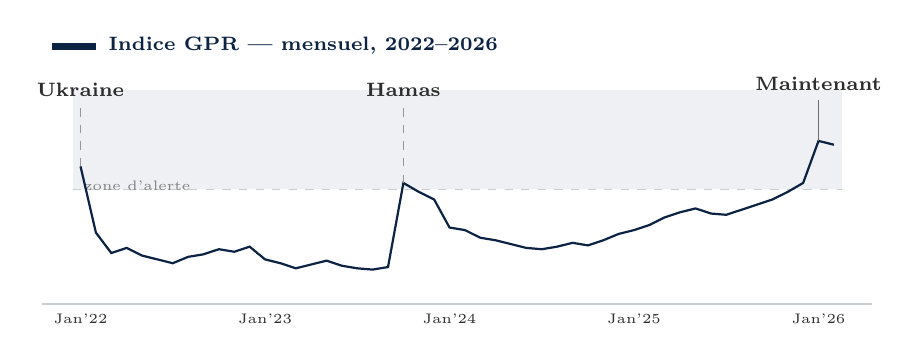
\begin{tikzpicture}
\begin{axis}[
  econ, height=4.3cm,
  title={\er Indice GPR — mensuel, 2022–2026},
  ytick={80,120,160,200},
  ymin=60, ymax=228,
  xtick={1,13,25,37,49},
  xticklabels={Jan'22,Jan'23,Jan'24,Jan'25,Jan'26},
  xmin=0.5, xmax=50.5,
]
%% Zone d'alerte haute (>150)
\fill[steel!15] (axis cs:0.5,150) rectangle (axis cs:50.5,228);
\draw[steel!50,thin,dashed] (axis cs:0.5,150) -- (axis cs:50.5,150);
\node[font=\tiny,coal!60,anchor=west] at (axis cs:0.6,153) {zone d'alerte};
%% GPR data Jan 2022 – Feb 2026 (source: Caldara & Iacoviello)
\addplot[navy,thick,mark=none] coordinates {
  (1,168)(2,116)(3,100)(4,104)
  (5, 98)(6, 95)(7, 92)(8, 97)
  (9, 99)(10,103)(11,101)(12,105)
  (13,95)(14,92)(15,88)(16,91)
  (17,94)(18,90)(19,88)(20,87)
  (21,89)(22,155)(23,148)(24,142)
  (25,120)(26,118)(27,112)(28,110)
  (29,107)(30,104)(31,103)(32,105)
  (33,108)(34,106)(35,110)(36,115)
  (37,118)(38,122)(39,128)(40,132)
  (41,135)(42,131)(43,130)(44,134)
  (45,138)(46,142)(47,148)(48,155)
  (49,188)(50,185)
};
\draw[coal!50,thin,dashed]
  (axis cs:1,168) -- (axis cs:1,215)
  node[anchor=south,font=\scriptsize\bfseries,coal]{Ukraine};
\draw[coal!50,thin,dashed]
  (axis cs:22,155) -- (axis cs:22,215)
  node[anchor=south,font=\scriptsize\bfseries,coal]{Hamas};
\draw[coal!70,thin]
  (axis cs:49,188) -- (axis cs:49,220)
  node[anchor=south,font=\scriptsize\bfseries,coal]{Maintenant};
\end{axis}
\end{tikzpicture}
\src{Caldara \& Iacoviello, GPR Index (matteoiacoviello.com).
Janv.\,2022\,=\,168 ; Oct.\,2023\,$\approx$\,155 ; Janv.\,2026\,$\approx$\,185–190.}
\end{column}

\end{columns}
\end{frame}


%%% ═══════════════════════════════════════════════════════════════════════════
%%% 02b · TRANSITION — BASCULE STRUCTURELLE
%%% ═══════════════════════════════════════════════════════════════════════════
\begin{frame}{... qui une bascule — le monde se réorganise en deux blocs}
\vspace{4pt}
\begin{columns}[T,totalwidth=\textwidth]

\begin{column}{0.46\textwidth}
\kw{Ce que le bruit masque.}
{\small Les conflits, les sanctions et la volatilité des marchés sont
visibles. Mais ils sont les symptômes d'un mouvement plus profond :
la fragmentation de l'ordre économique mondial en deux sphères
d'influence distinctes.}

\vspace{5pt}
\kw{La vraie rupture.}
{\small Depuis 2022, les échanges, les chaînes d'approvisionnement,
les monnaies de réserve et les normes technologiques se réorganisent
le long d'une ligne de fracture Est–Ouest. Ce n'est pas un cycle —
c'est un changement de régime.}

\vspace{5pt}
\kw{Ce que cela implique.}
{\small Les actifs, les secteurs et les géographies qui s'inscrivent
dans cette nouvelle géographie du pouvoir — défense, ressources
critiques, hubs régionaux — captent une prime structurelle durable.}
\end{column}

\begin{column}{0.04\textwidth}\end{column}

\begin{column}{0.50\textwidth}
\vspace{4pt}
\begin{tikzpicture}[
  bloc/.style={rectangle,draw=navy,fill=white,line width=0.8pt,
               font=\small\bfseries\color{navy},
               inner sep=6pt, minimum width=3.0cm, align=center},
  tag/.style={rectangle,draw=steel!60,fill=white,line width=0.4pt,
              font=\tiny\color{coal},
              inner sep=4pt, text width=2.85cm, align=left},
  node distance=0.3cm,
]
  %% Bloc Ouest
  \node[bloc](W){Bloc Occidental};
  \node[tag,below=0.2cm of W](TW)
    {OTAN élargi · dollar · semi-conducteurs · normes tech occidentales};

  %% Bloc Est
  \node[bloc,right=0.45cm of W](E){Bloc Oriental};
  \node[tag,below=0.2cm of E](TE)
    {BRICS+ · yuan · matières premières · normes tech alternatives};

  %% Fracture line
  \draw[coal!50, line width=1pt, dashed]
    ([yshift=6pt]W.north east) -- ([yshift=-6pt]W.south east);

  %% Zone pivot label
  \node[rectangle,draw=steel!40,fill=white,line width=0.4pt,
        font=\tiny\color{steel},inner sep=4pt,
        below=0.55cm of TW.south east, anchor=north]
    {Zones pivot : Golfe · ASEAN · Afrique};
\end{tikzpicture}

\vspace{6pt}
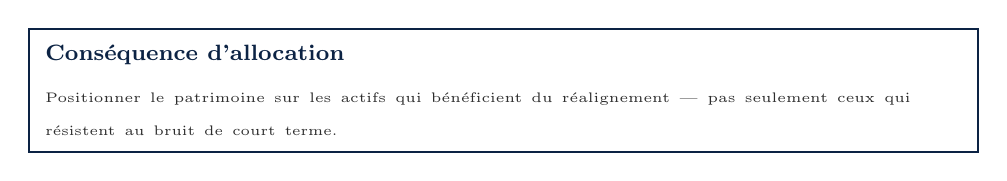
\begin{tikzpicture}
\node[draw=navy,fill=white,line width=0.8pt,inner sep=6pt,
      text width={\dimexpr\linewidth-14pt\relax},align=left]{%
  {\footnotesize\bfseries\color{navy}Conséquence d'allocation}\\[3pt]
  {\tiny\color{coal}Positionner le patrimoine sur les actifs
  qui bénéficient du réalignement — pas seulement ceux qui
  résistent au bruit de court terme.}};
\end{tikzpicture}
\end{column}

\end{columns}
\end{frame}

%%% ═══════════════════════════════════════════════════════════════════════════
%%% 02 · LES ACTIFS DE STABILITÉ
%%% ═══════════════════════════════════════════════════════════════════════════
\begin{frame}{Les actifs de stabilité — Or, sécurité, cybersécurité}
\begin{columns}[T,totalwidth=\textwidth]

\begin{column}{0.44\textwidth}
\vspace{4pt}
\kw{Rôle de l'or.}
{\small L'or préserve la valeur face aux dépréciations monétaires, à
l'inflation et aux crises systémiques. +27\,\% en 2024, +28\,\% en 2025.}

\vspace{5pt}
\kw{Allocation de protection.}
{\small Une exposition à l'or réduit la corrélation et amortit les chocs
sur les devises et les marchés obligataires. Gestion du risque, pas spéculation.}

\vspace{5pt}
\kw{Cybersécurité.}
{\small Protection des actifs numériques (comptes, identité, données bancaires) :
une composante à part entière de la gestion patrimoniale en 2026.}
\end{column}

\begin{column}{0.02\textwidth}\end{column}

\begin{column}{0.54\textwidth}
%% Gold price line chart (annual average USD/oz, 2018–2026)
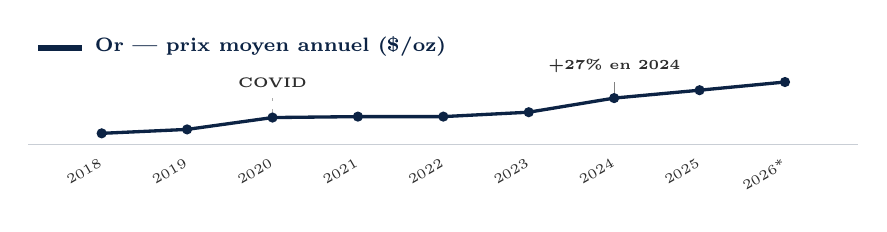
\begin{tikzpicture}
\begin{axis}[
  econ, height=2.5cm,
  title={\er Or — prix moyen annuel (\$/oz)},
  ytick={1000,1500,2000,2500,3000},
  ymin=900, ymax=3200,
  xtick={1,2,3,4,5,6,7,8,9},
  xticklabels={2018,2019,2020,2021,2022,2023,2024,2025,2026*},
  xmin=0.5, xmax=9.5,
  every x tick label/.style={font=\tiny,rotate=30,anchor=north east},
]
\addplot[navy,very thick,mark=*,mark options={fill=navy,scale=0.6}] coordinates {
  (1,1268)(2,1393)(3,1770)(4,1800)(5,1800)(6,1940)(7,2389)(8,2640)(9,2900)
};
\draw[coal!40,thin,dashed]
  (axis cs:3,1770) -- (axis cs:3,2400)
  node[anchor=south,font=\tiny\bfseries,coal]{COVID};
\draw[coal!60,thin]
  (axis cs:7,2389) -- (axis cs:7,2900)
  node[anchor=south,font=\tiny\bfseries,coal]{+27\% en 2024};
\end{axis}
\end{tikzpicture}
\src{LBMA Gold Price. 2026* = cours spot indicatif mars 2026 ($\approx$\,\$2\,900/oz).}

\vspace{3pt}
%% Cyber protection box — outline only, no fill
\begin{tikzpicture}
\node[draw=navy,fill=white,line width=0.8pt,inner sep=9pt,
      text width={\dimexpr\linewidth-18pt\relax},align=left]{%
  {\color{navy}\footnotesize\bfseries Protection du patrimoine numérique}\\[4pt]
  {\tiny\color{coal}%
  Données bancaires · Identité · Accès aux comptes · Fraudes \& phishing.
  La surface d'attaque des patrimoines numériques s'élargit chaque année.
  Une stratégie cyber fait partie d'une allocation patrimoniale rigoureuse.}};
\end{tikzpicture}
\end{column}

\end{columns}
\end{frame}

%%% ═══════════════════════════════════════════════════════════════════════════
%%% 03 · DÉFENSE EUROPÉENNE
%%% ═══════════════════════════════════════════════════════════════════════════
\begin{frame}{Défense européenne — Un investissement structurel}
\begin{columns}[T,totalwidth=\textwidth]

\begin{column}{0.44\textwidth}
\kw{Question d'allocation.}
{\small Le périmètre de la défense s'est élargi : satellites, cyberdéfense,
souveraineté industrielle. Ce segment va bien au-delà de l'armement classique
et présente un profil de risque distinct.}

\vspace{5pt}
\kw{Données 2026.}
{\small Les alliés OTAN ont dépassé les 2\,\% du PIB pour la première fois.
La Pologne atteint 4,1\,\% — un niveau historique. Les engagements sont
pluriannuels, validés par les parlements nationaux.}

\vspace{5pt}
\kw{Visibilité long terme.}
{\small Les budgets sont votés sur 10 ans avec peu de réversibilité
politique. Cette visibilité des flux de commandes est rare dans
un environnement macro incertain.}
\end{column}

\begin{column}{0.02\textwidth}\end{column}

\begin{column}{0.54\textwidth}
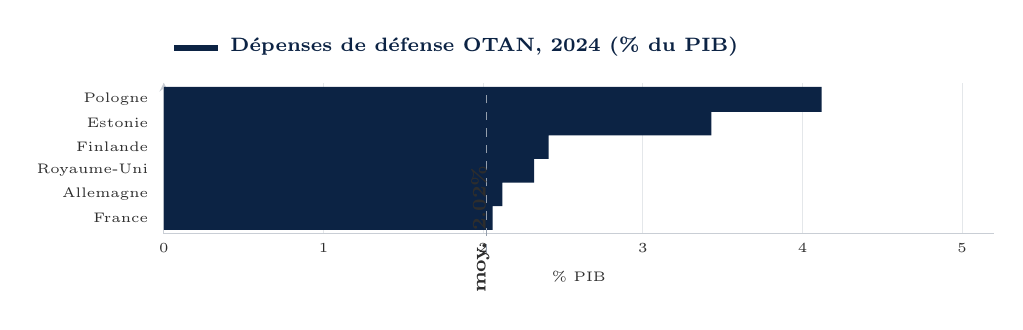
\begin{tikzpicture}
\begin{axis}[
  econh, height=3.5cm,
  title={\er Dépenses de défense OTAN, 2024 (\% du PIB)},
  xlabel={\% PIB},
  xlabel style={font=\tiny},
  ytick={1,2,3,4,5,6},
  yticklabels={France,Allemagne,Royaume-Uni,Finlande,Estonie,Pologne},
  xmin=0, xmax=5.2,
  xtick={0,1,2,3,4,5},
  bar width=9pt,
  enlarge y limits=0.14,
]
\addplot[fill=navy,draw=none] coordinates {
  (2.06,1)(2.12,2)(2.32,3)(2.41,4)(3.43,5)(4.12,6)
};
%% EU average line
\draw[steel,thin,dashed]
  (axis cs:2.02,-0.5) -- (axis cs:2.02,6.5);
\node[font=\scriptsize\bfseries,coal,rotate=90,anchor=south] at (axis cs:2.10,0.5)
  {moy. 2.02\%};
\end{axis}
\end{tikzpicture}
\src{NATO Defence Expenditure (août 2025). Moyenne UE-OTAN 2024\,=\,2.02\,\% (première fois confirmée).}
\begin{tikzpicture}
\node[draw=navy,fill=white,line width=0.8pt,inner sep=5pt,
      text width={\dimexpr\linewidth-16pt\relax},align=center]{%
  {\small\bfseries\color{navy}Budgets défense signés sur 10 ans}\\[3pt]
  {\tiny\color{coal}Technologie · Satellites · Cyberdéfense · Souveraineté}};
\end{tikzpicture}
\end{column}

\end{columns}
\end{frame}

%%% ═══════════════════════════════════════════════════════════════════════════
%%% 04 · LES NOUVELLES ZONES DE CROISSANCE
%%% ═══════════════════════════════════════════════════════════════════════════
\begin{frame}{Les nouvelles zones de croissance — Vietnam, Afrique minière}
\begin{columns}[T,totalwidth=\textwidth]

\begin{column}{0.44\textwidth}
\vspace{6pt}
\kw{Vietnam.}
{\small Réallocation industrielle accélérée par les tensions sino-américaines.
Manufactures, semi-conducteurs, électronique de consommation — des flux
d'investissements directs en forte progression.}

\vspace{9pt}
\kw{Afrique minière — Congo, Zambie.}
{\small Accès aux métaux critiques (cuivre, cobalt) indispensables à la
transition énergétique et aux chaînes d'approvisionnement technologiques.
La demande structurelle dépasse l'offre disponible à horizon 10 ans.}

\vspace{9pt}
{\tiny\color{steel}\itshape
Corridor Lobito : 6\,Mrd\$ d'engagements confirmés (UE, États-Unis,
partenaires). Relie les mines du Katanga aux ports de l'Atlantique.}
\end{column}

\begin{column}{0.02\textwidth}\end{column}

\begin{column}{0.54\textwidth}
\vspace{4pt}
\begin{tikzpicture}[
  loc/.style={rectangle,draw=navy,fill=white,line width=0.8pt,
              font=\small\bfseries\color{navy},inner sep=6pt,
              minimum width=2.8cm,align=center},
  desc/.style={rectangle,draw=steel!60,fill=white,line width=0.4pt,
               font=\tiny\color{coal},inner sep=6pt,
               text width=3.65cm,align=left},
  node distance=0.4cm and 0.25cm,
]
  \node[loc](V) {Vietnam};
  \node[desc,right=0.2cm of V](DV)
    {Atelier du monde · Samsung · supply chain délocalisée · croissance +7\,\%};

  \node[loc,below=0.55cm of V](A) {Congo · Zambie};
  \node[desc,right=0.2cm of A](DA)
    {Cuivre · Cobalt · Sans eux, pas de batteries ni d'énergie verte};

  \node[loc,below=0.55cm of A](L) {Corridor Lobito};
  \node[desc,right=0.2cm of L](DL)
    {6\,Mrd\$ engagés · Axe Atlantique–Katanga · UE \& partenaires};

  \node[loc,below=0.55cm of L](G) {Golfe \& ASEAN};
  \node[desc,right=0.2cm of G](DG)
    {Hubs digitaux · Finance islamique · Souveraineté technologique};
\end{tikzpicture}
\end{column}

\end{columns}
\end{frame}

%%% ═══════════════════════════════════════════════════════════════════════════
%%% 05 · SECTEURS À ÉVITER
%%% ═══════════════════════════════════════════════════════════════════════════
\begin{frame}{Les secteurs à éviter — Dette, logistique, vulnérabilité énergétique}
\begin{columns}[T,totalwidth=\textwidth]

\begin{column}{0.44\textwidth}
\vspace{3pt}
\kw{Dépendance structurelle à la Chine.}
{\small Les entreprises exposées aux disruptions de supply chains
subissent des coûts de transition élevés. La réorganisation logistique
en cours pénalise ceux qui tardent à s'adapter.}

\vspace{9pt}
\kw{Vulnérabilité énergétique et logistique.}
{\small Le renchérissement du fret et de l'énergie comprime les marges
des activités intensives en transport international.
L'impact est asymétrique et durable.}

\vspace{9pt}
\kw{Orientation recommandée.}
{\small Privilégier les secteurs locaux, digitaux et technologiques :
moins exposés aux aléas logistiques, plus de valeur ajoutée par unité
de capital engagé, meilleure résilience de marges.}
\end{column}

\begin{column}{0.02\textwidth}\end{column}

\begin{column}{0.54\textwidth}
\vspace{6pt}
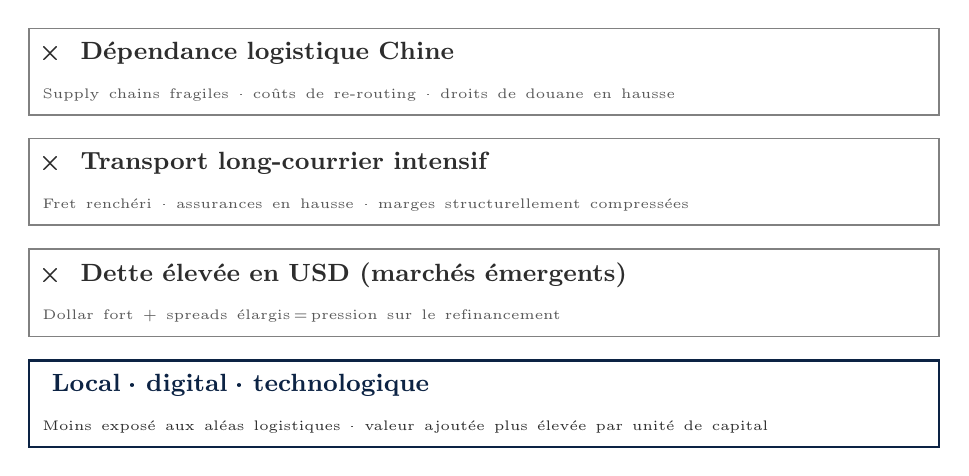
\begin{tikzpicture}[
  avoid/.style={rectangle,draw=coal!60,fill=white,line width=0.6pt,
                inner sep=5pt,
                text width={\dimexpr\linewidth-26pt\relax},align=left},
  ok/.style={rectangle,draw=navy,fill=white,line width=0.8pt,
             inner sep=5pt,
             text width={\dimexpr\linewidth-26pt\relax},align=left},
]
  \node[avoid](A){%
    {\color{coal}\bfseries\small\texttimes\ \ Dépendance logistique Chine}\\[2pt]
    {\tiny\color{coal!80}Supply chains fragiles · coûts de re-routing · droits de douane en hausse}};

  \node[avoid,below=0.28cm of A](B){%
    {\color{coal}\bfseries\small\texttimes\ \ Transport long-courrier intensif}\\[2pt]
    {\tiny\color{coal!80}Fret renchéri · assurances en hausse · marges structurellement compressées}};

  \node[avoid,below=0.28cm of B](C){%
    {\color{coal}\bfseries\small\texttimes\ \ Dette élevée en USD (marchés émergents)}\\[2pt]
    {\tiny\color{coal!80}Dollar fort + spreads élargis\,=\,pression sur le refinancement}};

  \node[ok,below=0.28cm of C](D){%
    {\color{navy}\bfseries\small \checkmark \ Local · digital · technologique}\\[2pt]
    {\tiny\color{coal}Moins exposé aux aléas logistiques · valeur ajoutée plus élevée par unité de capital}};
\end{tikzpicture}
\end{column}

\end{columns}
\end{frame}

%%% ═══════════════════════════════════════════════════════════════════════════
%%% 06 · SÉLECTION 2026
%%% ═══════════════════════════════════════════════════════════════════════════
\begin{frame}{Sélection 2026 — Les thèmes solides pour les années à venir}
\vspace{4pt}
\renewcommand{\arraystretch}{1.3}
\setlength{\tabcolsep}{6pt}
\begin{tabular}{>{\small\bfseries}p{3.2cm}%
                >{\footnotesize}p{7.0cm}%
                >{\small\bfseries\color{navy}}p{2.0cm}}
  \rowcolor{navy}
    {\color{white}Classe d'actif} &
    {\color{white}Thèse d'investissement} &
    {\color{white}Horizon} \\
  \rowcolor{steel!12}
    \color{navy}Or \& Argent &
    Réserve de valeur non corrélée. Protection contre l'inflation et
    les crises monétaires. Performance confirmée 2024–2025. &
    Structurel \\
  \color{navy}Défense Tech (Europe) &
    Budgets pluriannuels votés. Périmètre élargi : cyber, satellites,
    souveraineté industrielle. Visibilité de commandes rare. &
    5–10 ans \\
  \rowcolor{steel!12}
    \color{navy}Mines africaines &
    Métaux critiques (cuivre, cobalt) en déficit d'offre structurel.
    Demande portée par la transition énergétique mondiale. &
    10 ans \\
  \color{navy}Luxe \& IA &
    Résilience structurelle aux cycles économiques. Portés par la
    croissance des grandes fortunes et le déploiement de l'IA. &
    Long terme \\
\end{tabular}

\vspace{5pt}

\begin{tikzpicture}
\node[draw=navy,fill=white,line width=0.8pt,inner sep=6pt,
      text width={\dimexpr\textwidth-12pt\relax},align=center]{%
  \setlength{\tabcolsep}{10pt}
  \begin{tabular}{@{}cccc@{}}
    {\small\bfseries\color{navy}Or} &
    {\small\bfseries\color{navy}Défense} &
    {\small\bfseries\color{navy}Mines} &
    {\small\bfseries\color{navy}Luxe \& IA} \\
    {\tiny\color{steel}Protection} &
    {\tiny\color{steel}Souveraineté} &
    {\tiny\color{steel}Ressources} &
    {\tiny\color{steel}Croissance} \\
  \end{tabular}};
\end{tikzpicture}
\end{frame}

%%% ═══════════════════════════════════════════════════════════════════════════
%%% 07 · ALLOCATION 2026
%%% ═══════════════════════════════════════════════════════════════════════════
\begin{frame}{Allocation 2026 — Ancré en Afrique, ouvert sur le monde}
\begin{columns}[T,totalwidth=\textwidth]

\begin{column}{0.40\textwidth}
\centering\vspace{8pt}
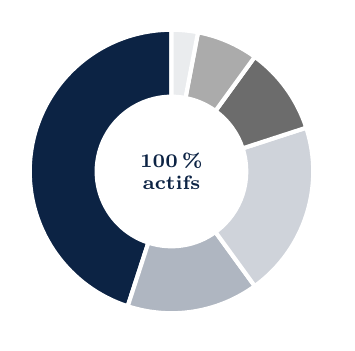
\begin{tikzpicture}
  \def\R{1.8}
  \def\r{0.95}
  %% 45 % Cœur Global      90°→252°
  \filldraw[fill=navy,     draw=white,line width=1.5pt]
    (90:\R) arc(90:252:\R) -- (252:\r) arc(252:90:\r) -- cycle;
  %% 15 % Économies afric. 252°→306°
  \filldraw[fill=steel!75, draw=white,line width=1.5pt]
    (252:\R) arc(252:306:\R) -- (306:\r) arc(306:252:\r) -- cycle;
  %% 20 % Ressources crit. 306°→378° (=18°)
  \filldraw[fill=steel!45, draw=white,line width=1.5pt]
    (306:\R) arc(306:378:\R) -- (378:\r) arc(378:306:\r) -- cycle;
  %% 10 % Défense          18°→54°
  \filldraw[fill=coal!70,  draw=white,line width=1.5pt]
    (18:\R) arc(18:54:\R) -- (54:\r) arc(54:18:\r) -- cycle;
  %% 7 % Tech & Cyber      54°→79.2°
  \filldraw[fill=coal!40,  draw=white,line width=1.5pt]
    (54:\R) arc(54:79.2:\R) -- (79.2:\r) arc(79.2:54:\r) -- cycle;
  %% 3 % Or & Argent       79.2°→90°
  \filldraw[fill=steel!20, draw=white,line width=1.5pt]
    (79.2:\R) arc(79.2:90:\R) -- (90:\r) arc(90:79.2:\r) -- cycle;
  %% Center
  \node[font=\scriptsize\bfseries\color{navy},align=center] {100\,\%\\actifs};
\end{tikzpicture}

\vspace{4pt}
{\tiny\color{steel}\itshape ETF liquides · horizon 5–10 ans}
\end{column}

\begin{column}{0.02\textwidth}\end{column}

\begin{column}{0.58\textwidth}
\vspace{3pt}

{\color{navy}\rule{7pt}{7pt}}\enspace
  {\small\bfseries\color{navy}45\,\%\ Cœur Global}\enspace{\tiny\color{steel}ACWI · VWRA}\\[-1pt]
{\tiny\color{coal!70}\hspace{10pt}Diversification mondiale · socle du portefeuille}\\[4pt]

{\color{steel!75}\rule{7pt}{7pt}}\enspace
  {\small\bfseries\color{navy}15\,\%\ Économies africaines}\enspace{\tiny\color{steel}AFK · FM}\\[-1pt]
{\tiny\color{coal!70}\hspace{10pt}Urbanisation · fintech · consommation}\\[4pt]

{\color{steel!45}\rule{7pt}{7pt}}\enspace
  {\small\bfseries\color{navy}20\,\%\ Ressources critiques}\enspace{\tiny\color{steel}COPX · REMX · LIT}\\[-1pt]
{\tiny\color{coal!70}\hspace{10pt}Cuivre · cobalt · lithium — transition énergétique}\\[4pt]

{\color{coal!70}\rule{7pt}{7pt}}\enspace
  {\small\bfseries\color{navy}10\,\%\ Défense \& Souveraineté}\enspace{\tiny\color{steel}XAR · EUAD}\\[-1pt]
{\tiny\color{coal!70}\hspace{10pt}Budgets votés sur 10 ans · visibilité des flux}\\[4pt]

{\color{coal!40}\rule{7pt}{7pt}}\enspace
  {\small\bfseries\color{navy}7\,\%\ Technologie \& Cyber}\enspace{\tiny\color{steel}CIBR · QQQ}\\[-1pt]
{\tiny\color{coal!70}\hspace{10pt}IA · cloud · sécurité numérique}\\[4pt]

{\color{steel!20}\rule{7pt}{7pt}}\enspace
  {\small\bfseries\color{navy}3\,\%\ Or \& Argent}\enspace{\tiny\color{steel}GLD · IAU · SIVR}\\[-1pt]
{\tiny\color{coal!70}\hspace{10pt}Protection monétaire · réserve de valeur}\\[5pt]

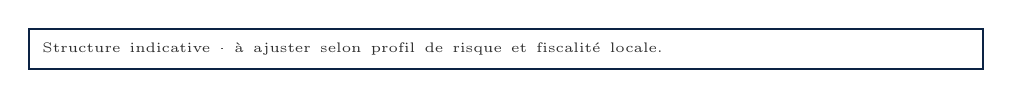
\begin{tikzpicture}
\node[draw=navy,fill=white,line width=0.7pt,inner sep=5pt,
      text width={\dimexpr\linewidth-10pt\relax},align=left]{%
  {\tiny\color{coal}Structure indicative · à ajuster selon profil de risque et fiscalité locale.}};
\end{tikzpicture}

\end{column}
\end{columns}
\end{frame}

\end{document}
